 
%Juan Luis: Incluyo algunos templates de diapositivas

\section{Results at a glance}

%%%%%%%%%%%%%%%%%%%%%%%%%%%%%%%%%%%%%%%%%%%%%%%%%%
\begin{frame}{Gaps and clusters}

\begin{columns}
\column{.4\textwidth}
  \includegraphics<1>[width=4.5cm]{images/jambywaldec.png} 
  \includegraphics<2>[width=4.5cm]{images/spacediagram.png}

\column{.6\textwidth}
  
  \begin{itemize}
  \item DPCT dynamics resemble traffic jams.
  \item Gaps and clusters form spontaneously.
  \begin{itemize}
  	\item<2> $\frac{n}{Y}$ (Density)
  	\item<2> Movement criterion 
    \begin{itemize}
  		\item<2> Phenotype (Fitness) (f)
  		\item<2> Genotype (similarity) (s)
  		\item<2> Random (r)
    \end{itemize}  	
  	\item<2>  Cellular-Island Hybrid!? 
  \end{itemize}  
  \end{itemize}

\end{columns}

\end{frame}
%%%%%%%%%%%%%%%%%%%%%%%%%%%%%%%%%%%%%%%%%%%%%%%%%%
\note{Talk no more than 1 minute.}

%%%%%%%%%%%%%%%%%%%%%%%%%%%%%%%%%%%%%%%%%%%%%%%%%%
\begin{frame}{Results using trap functions}


\begin{columns}
\column{.75\textwidth}
\begin{scriptsize}
\begin{block}{Settings}
 \begin{itemize}
 \item $n=400$
 \item 2-trap $l=500$ 
 \item 3-trap $l=375$ 
 \item 4-trap $l=300$
 \item Top. (torus) (ring) (DPCT)
 \end{itemize}
\end{block}
\end{scriptsize}
\column{.25\textwidth}
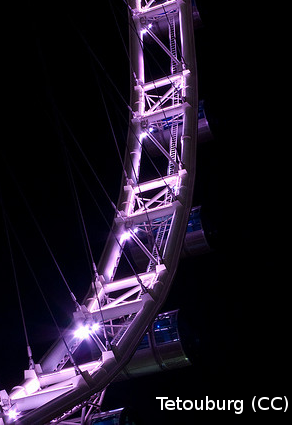
\includegraphics[width=2cm]{images/ringteutoburg.png} 
\end{columns}

\centering
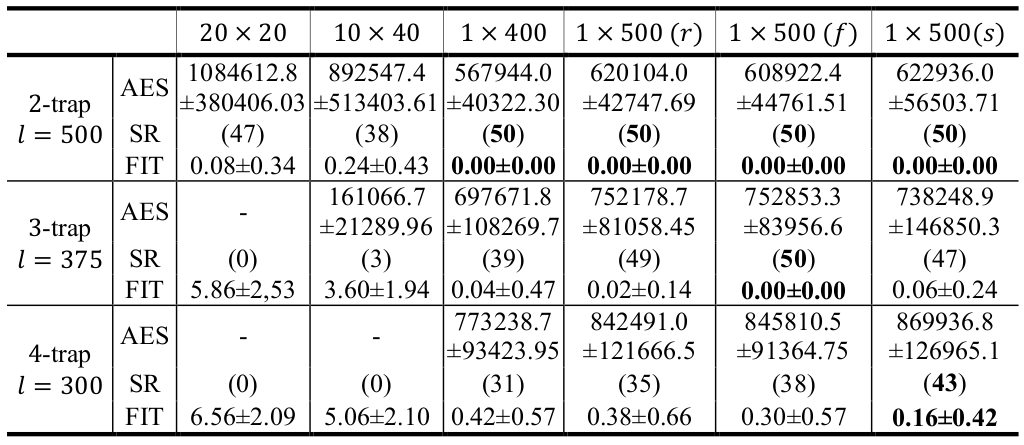
\includegraphics[width=9cm]{images/results1.png} 

\end{frame}
%%%%%%%%%%%%%%%%%%%%%%%%%%%%%%%%%%%%%%%%%%%%%%%%%%
\note{Talk no more than 1 minute.}

%%%%%%%%%%%%%%%%%%%%%%%%%%%%%%%%%%%%%%%%%%%%%%%%%%
\begin{frame}{Influence of density}
\begin{columns}
\column{.75\textwidth}
\begin{scriptsize}
\begin{block}{Settings}
 \begin{itemize}
 \item $n=400$
 \item 4-trap $l=300$
 \end{itemize}
\end{block}
\end{scriptsize}
\column{.25\textwidth}
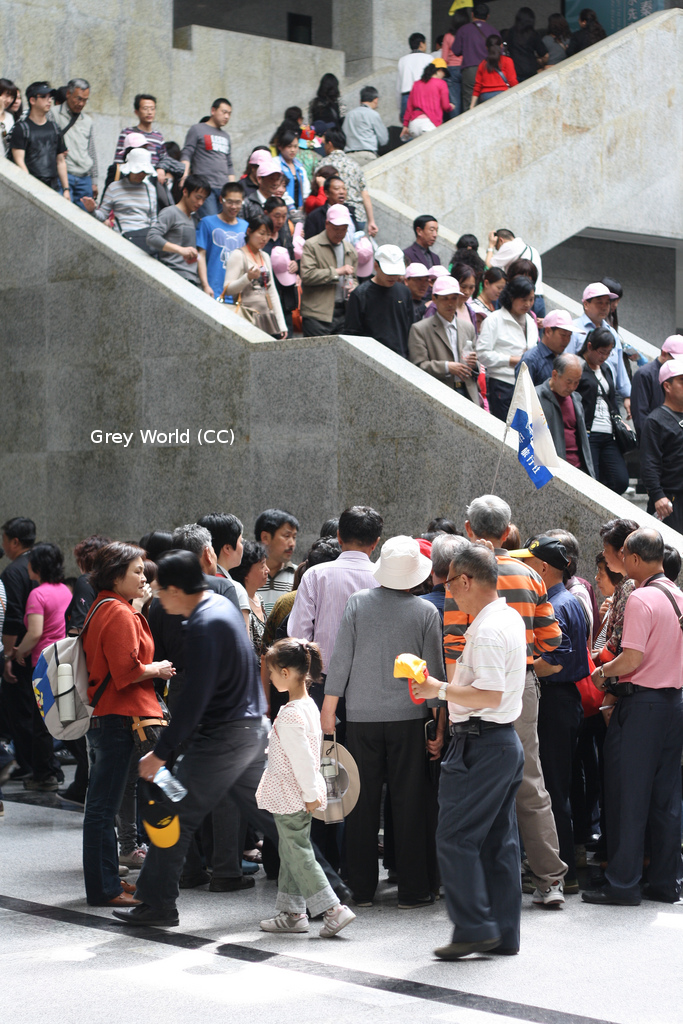
\includegraphics[width=2cm]{images/crowd.png} 

\end{columns}
\centering
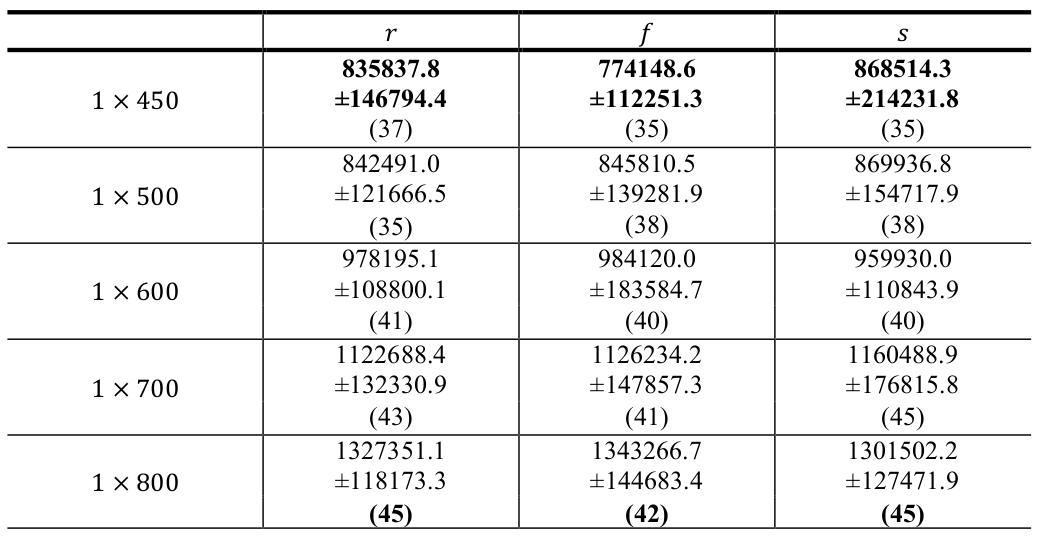
\includegraphics[width=8cm]{images/results2.png} 


\end{frame}
%%%%%%%%%%%%%%%%%%%%%%%%%%%%%%%%%%%%%%%%%%%%%%%%%%
\note{Talk no more than 1 minute.}


%%%%%%%%%%%%%%%%%%%%%%%%%%%%%%%%%%%%%%%%%%%%%%%%%%
\begin{frame}{What about optimal population sizes?}
\begin{columns}
\column{.75\textwidth}
\begin{scriptsize}
\begin{block}{Settings}
 \begin{itemize}
 \item \textst{n=400} $\rightarrow optimal$
 \item 4-trap 
 \end{itemize}
\end{block}
\end{scriptsize}
\column{.25\textwidth}
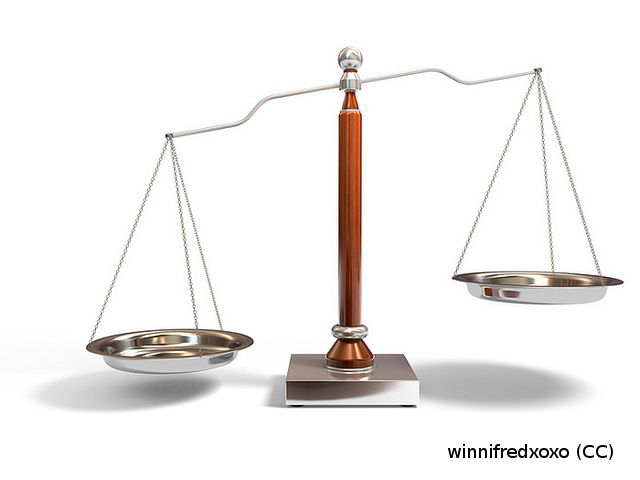
\includegraphics[width=2.5cm]{images/scale.png} 

\end{columns}
\centering
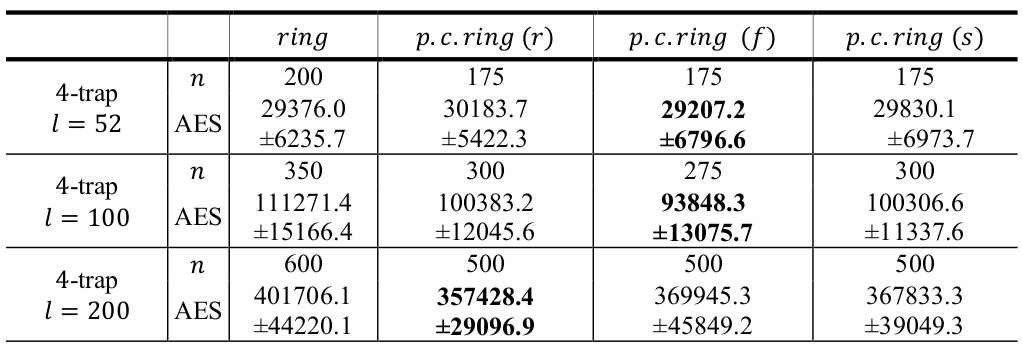
\includegraphics[width=10cm]{images/results3.png} 


\end{frame}
%%%%%%%%%%%%%%%%%%%%%%%%%%%%%%%%%%%%%%%%%%%%%%%%%%
\note{Talk no more than 1 minute.}



\section{Conclusions}

%%%%%%%%%%%%%%%%%%%%%%%%%%%%%%%%%%%%%%%%%%%%%%%%%%
\begin{frame}
\frametitle{Conclusions}

\begin{itemize}
\item Partially connected 1-dimensional cellular GA
\item The resulting structure displays an island-model behaviour 
\item Promotion of genetic diversity and reduction of the minimum population size
\end{itemize}

\only<2>{
\begin{block}{Future works}
 \begin{itemize}
 \item Extension to 2-dimensional model
 \item Modelling the DPCT in a probability-based model
 \end{itemize}
\end{block}
}
\end{frame}
%%%%%%%%%%%%%%%%%%%%%%%%%%%%%%%%%%%%%%%%%%%%%%%%%%
